% Options for packages loaded elsewhere
\PassOptionsToPackage{unicode}{hyperref}
\PassOptionsToPackage{hyphens}{url}
%
\documentclass[
]{article}
\usepackage{amsmath,amssymb}
\usepackage{lmodern}
\usepackage{float}
\usepackage{iftex}
\ifPDFTeX
  \usepackage[T1]{fontenc}
  \usepackage[utf8]{inputenc}
  \usepackage{textcomp} % provide euro and other symbols
\else % if luatex or xetex
  \usepackage{unicode-math}
  \defaultfontfeatures{Scale=MatchLowercase}
  \defaultfontfeatures[\rmfamily]{Ligatures=TeX,Scale=1}
\fi
% Use upquote if available, for straight quotes in verbatim environments
\IfFileExists{upquote.sty}{\usepackage{upquote}}{}
\IfFileExists{microtype.sty}{% use microtype if available
  \usepackage[]{microtype}
  \UseMicrotypeSet[protrusion]{basicmath} % disable protrusion for tt fonts
}{}
\makeatletter
\@ifundefined{KOMAClassName}{% if non-KOMA class
  \IfFileExists{parskip.sty}{%
    \usepackage{parskip}
  }{% else
    \setlength{\parindent}{0pt}
    \setlength{\parskip}{6pt plus 2pt minus 1pt}}
}{% if KOMA class
  \KOMAoptions{parskip=half}}
\makeatother
\usepackage{xcolor}
\IfFileExists{xurl.sty}{\usepackage{xurl}}{} % add URL line breaks if available
\IfFileExists{bookmark.sty}{\usepackage{bookmark}}{\usepackage{hyperref}}
\hypersetup{
  pdftitle={arc42 Template},
  hidelinks,
  pdfcreator={LaTeX via pandoc}}
\urlstyle{same} % disable monospaced font for URLs
\usepackage{longtable,booktabs,array}
\usepackage{calc} % for calculating minipage widths
% Correct order of tables after \paragraph or \subparagraph
\usepackage{etoolbox}
\makeatletter
\patchcmd\longtable{\par}{\if@noskipsec\mbox{}\fi\par}{}{}
\makeatother
% Allow footnotes in longtable head/foot
\IfFileExists{footnotehyper.sty}{\usepackage{footnotehyper}}{\usepackage{footnote}}
\makesavenoteenv{longtable}
\usepackage{graphicx}
\makeatletter
\def\maxwidth{\ifdim\Gin@nat@width>\linewidth\linewidth\else\Gin@nat@width\fi}
\def\maxheight{\ifdim\Gin@nat@height>\textheight\textheight\else\Gin@nat@height\fi}
\makeatother
% Scale images if necessary, so that they will not overflow the page
% margins by default, and it is still possible to overwrite the defaults
% using explicit options in \includegraphics[width, height, ...]{}
\setkeys{Gin}{width=\maxwidth,height=\maxheight,keepaspectratio}
% Set default figure placement to htbp
\makeatletter
\def\fps@figure{htbp}
\makeatother
\setlength{\emergencystretch}{3em} % prevent overfull lines
\providecommand{\tightlist}{%
  \setlength{\itemsep}{0pt}\setlength{\parskip}{0pt}}
\setcounter{secnumdepth}{-\maxdimen} % remove section numbering
\ifLuaTeX
  \usepackage{selnolig}  % disable illegal ligatures
\fi

\title{RIOT: Flood Gate Management System}
\author{}
\date{May 2025}

\begin{document}
\maketitle

\section{}

\hypertarget{section-introduction-and-goals}{%
\section{Introduction and Goals}\label{section-introduction-and-goals}}
This project aims to develop a system capable of monitoring the state of flood gates in the Hamburg Harbor, which are safety-critical infrastructure, and to partically digitalize the current analog workflow.

%\newpage
\hypertarget{_requirements_overview}{%
\subsection{Requirements Overview}\label{_requirements_overview}}
\subsubsection{MVP Requirements}
\renewcommand{\arraystretch}{1.5} % Erhöht den Zeilenabstand um 50%
\begin{longtable}[]{@{}
 >{\raggedright\arraybackslash}p{(\columnwidth - 4\tabcolsep) * \real{0.1000}}
 >{\raggedright\arraybackslash}p{(\columnwidth - 4\tabcolsep) * \real{0.4000}}
 >{\raggedright\arraybackslash}p{(\columnwidth - 4\tabcolsep) * \real{0.5000}}@{}}
\toprule
\begin{minipage}[b]{\linewidth}\raggedright
\textbf{Nr.}
\end{minipage} &
\begin{minipage}[b]{\linewidth}\raggedright
\textbf{Requirement}
\end{minipage} &
\begin{minipage}[b]{\linewidth}\raggedright
\textbf{Description}
\end{minipage} \\
\midrule
\endhead
MR01 & Signal gate open/closed & The system shall be able to signal whether a gate is currently open or closed. \\
MR02 & Request gate open/close to GateMate & The system shall allow the pilot to request a gate to open or close. \\
MR03 & Visualize gate state & The system shall provide visual indication of the current gate state. \\
MR04 & Manual state switch & The SenseMate shall be able to manually override the gate state when necessary. \\
MR05 & Secure Communication & All communication regarding gate state shall be secured and encrypted. \\
MR06 & State information exchange between Sense- and GateMate & The system shall facilitate state information exchange between SenseMate and GateMate. \\
MR07 & Periodic Server Update about the state of the gate & The Sense- and GateMate shall send periodic updates to the server about gate state. \\
MR08 & Track state of a gate & The Server shall maintain a history of the current gate state and state changes. \\
MR09 & Display gate information on SenseMate & The SenseMate component shall display relevant gate information to the workers. \\
MR10 & Request gate open/close to SenseMate & The system shall allow the pilot to assign a SenseMate to open/close specific gates.\\
\bottomrule
\caption{Requirements for MVP}\\
\end{longtable}

%\newpage
\subsubsection{Optional Requirements}
\begin{longtable}[]{@{}
 >{\raggedright\arraybackslash}p{(\columnwidth - 4\tabcolsep) * \real{0.1000}}
 >{\raggedright\arraybackslash}p{(\columnwidth - 4\tabcolsep) * \real{0.4000}}
 >{\raggedright\arraybackslash}p{(\columnwidth - 4\tabcolsep) * \real{0.5000}}@{}}
\toprule
\begin{minipage}[b]{\linewidth}\raggedright
\textbf{Nr.}
\end{minipage} &
\begin{minipage}[b]{\linewidth}\raggedright
\textbf{Requirement}
\end{minipage} &
\begin{minipage}[b]{\linewidth}\raggedright
\textbf{Description}
\end{minipage} \\
\midrule
\endhead
OR01 & Location Tracking of Sense- and GateMates & The system should be able to track and display the current location of the Sense- and GateMate. \\
OR02 & Smart assignment & The system shall provide a smart assignment functionality for efficient closing workflow. \\
OR03 & Battery State & The system shall be able to track and display the current battery state of the SenseMate. \\
OR04 & Cycle-Change & The system should be able to adjust the update frequency from MR07. \\
OR05 & Device Management & The system should be able to register/unregister devices dynamically. \\
OR06 & Waterproof case for the GateMates & \\
\bottomrule
\caption{Optional Requirements}\\
\end{longtable}


%\newpage
\hypertarget{_quality_goals}{%
\subsection{Quality Goals}\label{_quality_goals}}
\begin{longtable}[]{@{}
  >{\raggedright\arraybackslash}p{0.15\textwidth}
  >{\raggedright\arraybackslash}p{0.45\textwidth}
  >{\raggedright\arraybackslash}p{0.2\textwidth}
  >{\raggedright\arraybackslash}p{0.15\textwidth}@{}}
\toprule
\textbf{Goal} & \textbf{Description} & \textbf{Metric} & \textbf{Value} \\
\midrule
\endhead
Performance & The system must transmit gate status updates and operational commands with minimal latency to ensure timely response during flood events. & Transmission Time & \[ \geq 500ms \] \\
Reliability & The system must accurately communicate flood gate statuses with high precision to prevent false alarms or missed critical states. & Error Rate & \[ \leq 0.1\% \] \\
Scalability & The system should support automatic integration of new devices without requiring significant reconfiguration of the existing infrastructure. & Integration Time & \[ \leq 1 hour \] \\
Fault Tolerance & The system must detect malfunctioning components and provide alternative communication pathways when primary channels fail. & Recovery Time & \[ \leq 5 minutes \] \\
Availability & The system must maintain operational capability during emergency situations, including power outages and severe weather conditions. & Uptime & \[ \geq 99.99\% \] \\
Efficiency & The system should minimize power consumption to extend battery life during work hours. & Battery life for SenseMate & \[ \geq 12 hours \] \\
Usability & The system interface must be intuitive enough for operators to use the dashboard and report gate state during different weather situations. & - & - \\
\bottomrule
\caption{Quality Goals for Flood Gate Management System}\\
\end{longtable}

\newpage
\hypertarget{_stakeholders}{%
\subsection{Stakeholders}\label{_stakeholders}}

\begin{longtable}[]{@{}
  >{\raggedright\arraybackslash}p{(\columnwidth - 4\tabcolsep) * \real{0.2000}}
  >{\raggedright\arraybackslash}p{(\columnwidth - 4\tabcolsep) * \real{0.9000}}@{}}
\toprule
\begin{minipage}[b]{\linewidth}\raggedright
\textbf{Role/Name}
\end{minipage} & 
\begin{minipage}[b]{\linewidth}\raggedright
\textbf{Expectations}
\end{minipage} \\
\midrule
\endhead
Pilot & The Pilot is one of the main stakeholders with the following expectations:
\begin{itemize}
    \item Wants to know whether a gate has been closed or not
    \item Wants to be able to monitor the current state of the gate
    \item Wants to give instructions to close or open a gate
\end{itemize} \\\\
Worker & The Worker is another key stakeholder with the following expectations:
\begin{itemize}
    \item Wants to know whether they have actually closed the gate
    \item Wants an easy-to-use gadget
    \item Wants to be able to manually transfer the status of a gate
\end{itemize} \\\\
Rescuemate & Wants a solution for monitoring floodgates in the harbor \\
\bottomrule
\caption{Stakeholders}
\end{longtable}

\hypertarget{section-architecture-constraints}{%
\section{Architecture Constraints}\label{section-architecture-constraints}}
\begin{longtable}[]{@{}
  >{\raggedright\arraybackslash}p{(\columnwidth - 4\tabcolsep) * \real{0.4000}}
  >{\raggedright\arraybackslash}p{(\columnwidth - 4\tabcolsep) * \real{0.7000}}@{}}
\toprule
\begin{minipage}[b]{\linewidth}\raggedright
\textbf{Constraint}
\end{minipage} & 
\begin{minipage}[b]{\linewidth}\raggedright
\textbf{Description}
\end{minipage} \\
\midrule
\endhead

feather-nrf52840 board & Microcontroller for the Sense- and GateMates.\\
LoRaWAN Communication & The communication between the Nodes and the Server shall be over LoRaWAN protocol.\\
BLE & The communication between the Nodes shall be over BLE.\\
RIOT & The software of the Nodes shall be based on RIOT OS.\\

\bottomrule
\caption{Constraints}
\end{longtable}


\hypertarget{section-context-and-scope}{%
\section{Context and Scope}\label{section-context-and-scope}}


\begin{figure}[H]
  \centering
  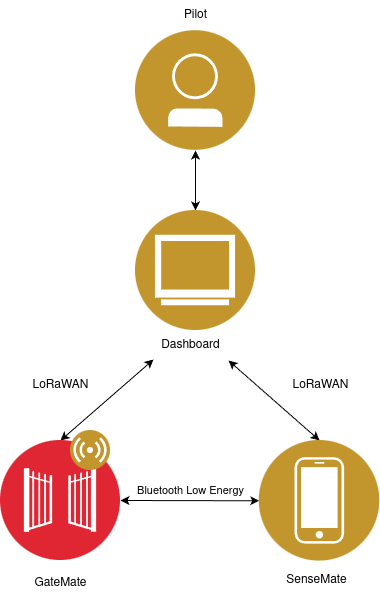
\includegraphics[width=1 \textwidth]{images/context-diagramm.png}
  \caption{Context}
  %\vspace{-130pt} 
  \label{fig:context}
  
\end{figure}



\hypertarget{_business_context}{%
\subsection{Business Context}\label{_business_context}}


\hypertarget{_technical_context}{%
\subsection{Technical Context}\label{_technical_context}}


\hypertarget{section-solution-strategy}{%
\section{Solution Strategy}\label{section-solution-strategy}}

\hypertarget{section-building-block-view}{%
\section{Building Block View}\label{section-building-block-view}}

\hypertarget{_whitebox_overall_system}{%
\subsection{Whitebox Overall System}\label{_whitebox_overall_system}}

\emph{\textbf{\textless Overview Diagram\textgreater{}}}

\begin{description}
\item[Motivation]
\emph{\textless text explanation\textgreater{}}
\item[Contained Building Blocks]
\emph{\textless Description of contained building block (black
boxes)\textgreater{}}
\item[Important Interfaces]
\emph{\textless Description of important interfaces\textgreater{}}
\end{description}

\hypertarget{__name_black_box_1}{%
\subsubsection{\textless Name black box
1\textgreater{}}\label{__name_black_box_1}}

\emph{\textless Purpose/Responsibility\textgreater{}}

\emph{\textless Interface(s)\textgreater{}}

\emph{\textless(Optional) Quality/Performance
Characteristics\textgreater{}}

\emph{\textless(Optional) Directory/File Location\textgreater{}}

\emph{\textless(Optional) Fulfilled Requirements\textgreater{}}

\emph{\textless(optional) Open Issues/Problems/Risks\textgreater{}}

\hypertarget{__name_black_box_2}{%
\subsubsection{\textless Name black box
2\textgreater{}}\label{__name_black_box_2}}

\emph{\textless black box template\textgreater{}}

\hypertarget{__name_black_box_n}{%
\subsubsection{\textless Name black box
n\textgreater{}}\label{__name_black_box_n}}

\emph{\textless black box template\textgreater{}}

\hypertarget{__name_interface_1}{%
\subsubsection{\textless Name interface
1\textgreater{}}\label{__name_interface_1}}

\ldots{}

\hypertarget{__name_interface_m}{%
\subsubsection{\textless Name interface
m\textgreater{}}\label{__name_interface_m}}

\hypertarget{_level_2}{%
\subsection{Level 2}\label{_level_2}}

\hypertarget{_white_box_emphasis_building_block_1_emphasis}{%
\subsubsection{\texorpdfstring{White Box \emph{\textless building block
1\textgreater{}}}{White Box \textless building block 1\textgreater{}}}\label{_white_box_emphasis_building_block_1_emphasis}}

\emph{\textless white box template\textgreater{}}

\hypertarget{_white_box_emphasis_building_block_2_emphasis}{%
\subsubsection{\texorpdfstring{White Box \emph{\textless building block
2\textgreater{}}}{White Box \textless building block 2\textgreater{}}}\label{_white_box_emphasis_building_block_2_emphasis}}

\emph{\textless white box template\textgreater{}}

\ldots{}

\hypertarget{_white_box_emphasis_building_block_m_emphasis}{%
\subsubsection{\texorpdfstring{White Box \emph{\textless building block
m\textgreater{}}}{White Box \textless building block m\textgreater{}}}\label{_white_box_emphasis_building_block_m_emphasis}}

\emph{\textless white box template\textgreater{}}

\hypertarget{_level_3}{%
\subsection{Level 3}\label{_level_3}}

\hypertarget{_white_box_building_block_x_1}{%
\subsubsection{White Box \textless\_building block
x.1\_\textgreater{}}\label{_white_box_building_block_x_1}}

\emph{\textless white box template\textgreater{}}

\hypertarget{_white_box_building_block_x_2}{%
\subsubsection{White Box \textless\_building block
x.2\_\textgreater{}}\label{_white_box_building_block_x_2}}

\emph{\textless white box template\textgreater{}}

\hypertarget{_white_box_building_block_y_1}{%
\subsubsection{White Box \textless\_building block
y.1\_\textgreater{}}\label{_white_box_building_block_y_1}}

\emph{\textless white box template\textgreater{}}

\hypertarget{section-runtime-view}{%
\section{Runtime View}\label{section-runtime-view}}

\begin{figure}[H]
  \centering
  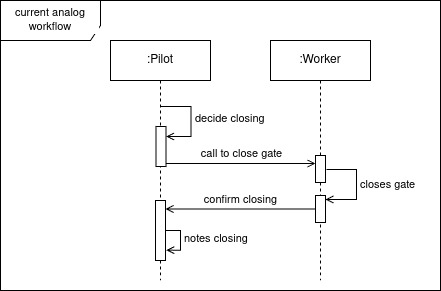
\includegraphics[width=0.7\textwidth]{images/sequence_diagram-current.jpg}
  \caption{sequence diagram of the current workflows}
  \label{fig:seq_intro_curr}
\end{figure}

\begin{figure}[H]
  \centering
  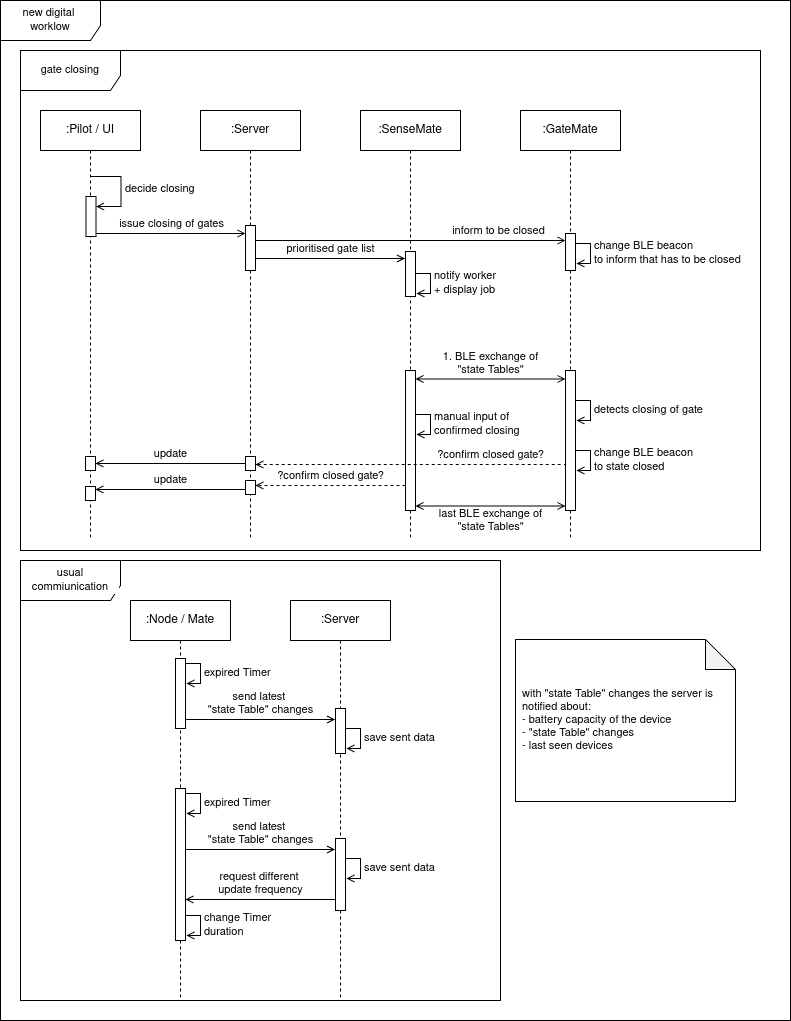
\includegraphics[width=\textwidth]{images/sequence_diagram-new.png}
  \caption{sequence diagram of the new workflows}
  \label{fig:seq_intro_new}
\end{figure}

\hypertarget{__runtime_scenario_1}{%
\subsection{\textless Runtime Scenario
1\textgreater{}}\label{__runtime_scenario_1}}

\begin{itemize}
\item
  \emph{\textless insert runtime diagram or textual description of the
  scenario\textgreater{}}
\item
  \emph{\textless insert description of the notable aspects of the
  interactions between the building block instances depicted in this
  diagram.\textgreater{}}
\end{itemize}

\hypertarget{__runtime_scenario_2}{%
\subsection{\textless Runtime Scenario
2\textgreater{}}\label{__runtime_scenario_2}}

\hypertarget{_}{%
\subsection{\ldots{}}\label{_}}

\hypertarget{__runtime_scenario_n}{%
\subsection{\textless Runtime Scenario
n\textgreater{}}\label{__runtime_scenario_n}}

\hypertarget{section-deployment-view}{%
\section{Deployment View}\label{section-deployment-view}}

\hypertarget{_infrastructure_level_1}{%
\subsection{Infrastructure Level 1}\label{_infrastructure_level_1}}

\emph{\textbf{\textless Overview Diagram\textgreater{}}}

\begin{description}
\item[Motivation]
\emph{\textless explanation in text form\textgreater{}}
\item[Quality and/or Performance Features]
\emph{\textless explanation in text form\textgreater{}}
\item[Mapping of Building Blocks to Infrastructure]
\emph{\textless description of the mapping\textgreater{}}
\end{description}

\hypertarget{_infrastructure_level_2}{%
\subsection{Infrastructure Level 2}\label{_infrastructure_level_2}}

\hypertarget{__emphasis_infrastructure_element_1_emphasis}{%
\subsubsection{\texorpdfstring{\emph{\textless Infrastructure Element
1\textgreater{}}}{\textless Infrastructure Element 1\textgreater{}}}\label{__emphasis_infrastructure_element_1_emphasis}}

\emph{\textless diagram + explanation\textgreater{}}

\hypertarget{__emphasis_infrastructure_element_2_emphasis}{%
\subsubsection{\texorpdfstring{\emph{\textless Infrastructure Element
2\textgreater{}}}{\textless Infrastructure Element 2\textgreater{}}}\label{__emphasis_infrastructure_element_2_emphasis}}

\emph{\textless diagram + explanation\textgreater{}}

\ldots{}

\hypertarget{__emphasis_infrastructure_element_n_emphasis}{%
\subsubsection{\texorpdfstring{\emph{\textless Infrastructure Element
n\textgreater{}}}{\textless Infrastructure Element n\textgreater{}}}\label{__emphasis_infrastructure_element_n_emphasis}}

\emph{\textless diagram + explanation\textgreater{}}

\hypertarget{section-concepts}{%
\section{Cross-cutting Concepts}\label{section-concepts}}

\hypertarget{__emphasis_concept_1_emphasis}{%
\subsection{\texorpdfstring{\emph{\textless Concept
1\textgreater{}}}{\textless Concept 1\textgreater{}}}\label{__emphasis_concept_1_emphasis}}

\emph{\textless explanation\textgreater{}}

\hypertarget{__emphasis_concept_2_emphasis}{%
\subsection{\texorpdfstring{\emph{\textless Concept
2\textgreater{}}}{\textless Concept 2\textgreater{}}}\label{__emphasis_concept_2_emphasis}}

\emph{\textless explanation\textgreater{}}

\ldots{}

\hypertarget{__emphasis_concept_n_emphasis}{%
\subsection{\texorpdfstring{\emph{\textless Concept
n\textgreater{}}}{\textless Concept n\textgreater{}}}\label{__emphasis_concept_n_emphasis}}

\emph{\textless explanation\textgreater{}}

\hypertarget{section-design-decisions}{%
\section{Architecture Decisions}\label{section-design-decisions}}

\hypertarget{section-quality-scenarios}{%
\section{Quality Requirements}\label{section-quality-scenarios}}

\hypertarget{_quality_tree}{%
\subsection{Quality Tree}\label{_quality_tree}}

\hypertarget{_quality_scenarios}{%
\subsection{Quality Scenarios}\label{_quality_scenarios}}

\hypertarget{section-technical-risks}{%
\section{Risks and Technical Debts}\label{section-technical-risks}}

\newpage
\hypertarget{section-glossary}{%
\section{Glossary}\label{section-glossary}}

\begin{longtable}[]{@{}
  >{\raggedright\arraybackslash}p{(\columnwidth - 2\tabcolsep) * \real{0.3333}}
  >{\raggedright\arraybackslash}p{(\columnwidth - 2\tabcolsep) * \real{0.6667}}@{}}
\toprule
\begin{minipage}[b]{\linewidth}\raggedright
\textbf{Term}
\end{minipage} & \begin{minipage}[b]{\linewidth}\raggedright
\textbf{Definition}
\end{minipage} \\
\midrule
\endhead
SenseMate & Device carried by the workers.\\
GateMate & Device that is attached to the flood gates and is responsible for reporting the gate state.\\
Node & Could be SenseMate or GateMate.\\
\bottomrule
\end{longtable}

\end{document}
